\documentclass[11pt]{article}

\usepackage[margin=1in]{geometry}
\usepackage{times}
\usepackage{microtype}
\usepackage{graphicx}
\usepackage{booktabs}
\usepackage{multirow}
\usepackage{amsmath}
\usepackage{enumitem}
\usepackage{hyperref}
\usepackage{xcolor}
\usepackage{caption}
\usepackage{subcaption}
\usepackage[numbers]{natbib}

\title{Prompt and Format Robustness in LLM Evaluation}
\author{
Capstone Advisor: Kai-Wei Chang\\[0.75em]
Allen Ma\\
M.S. Computer Science\\
University of California, Los Angeles
}
\date{}

\begin{document}
\maketitle

\begin{abstract}
Large language model (LLM) evaluations often report a single score obtained from a single prompt template, but recent work suggests that such scores can be sensitive to seemingly minor prompt-design choices. This project studies prompt and output-format robustness on two structured tasks: TREC-6 question classification and GSM8K grade-school math. I evaluate two modern OpenAI models, \texttt{gpt-5-nano} and \texttt{gpt-5-mini}, on 100 frozen examples per task using eight semantically equivalent prompt variants formed by crossing two instruction wordings with four output-format constraints. Each raw model output is scored twice: once with strict exact-format scoring and once with a deterministic equivalence-aware scorer that extracts and normalizes harmless answer-format variations. The main results show moderate prompt sensitivity: prompt accuracy ranges from 2--8 percentage points depending on task, model, and scorer. Equivalence-aware scoring reduces GSM8K prompt sensitivity by 1 percentage point for both models and increases average GSM8K accuracy by recovering benign numeric formatting differences such as \texttt{5.00} versus \texttt{5}. TREC-6 shows essentially no strict-versus-equivalence scoring gap, because model outputs are typically valid labels or genuinely wrong labels. As a secondary validation, a \texttt{gpt-5.4} judge audited all 326 outputs that failed strict scoring and agreed exactly with the deterministic equivalence-aware scorer. These findings support the view that prompt sensitivity is present but modest in this controlled setting, and that scoring artifacts matter most when task outputs admit harmless surface-form variation.
\end{abstract}

\section{Introduction}

LLM evaluation is often treated as if a model-task pair has a stable scalar performance value. In practice, prompting-based evaluation introduces an additional choice: the prompt template. Prior work has shown that prompt formatting and instruction wording can substantially change measured model performance even when the underlying task and examples remain fixed \citep{sclar2024sensitivity,mizrahi2024state}. This makes single-prompt evaluation fragile: a reported score may partly reflect the arbitrary prompt selected by the evaluator.

Recent work further argues that some measured prompt sensitivity may be an evaluation artifact rather than pure model brittleness. In particular, rigid exact-match or heuristic scoring can mark semantically correct outputs as wrong when the model uses a different but equivalent surface form \citep{hua2025flaw}. For example, if the gold answer is \texttt{5}, the output \texttt{The answer is 5.00} may be semantically correct but fail a strict string match. If different prompts systematically elicit different output styles, apparent prompt sensitivity may partly reflect scoring brittleness.

This project tests that issue in a small, controlled empirical setting. I evaluate two modern OpenAI models on two structured tasks under a fixed family of semantically equivalent prompts. The prompts vary along two axes: instruction wording and output-format constraint. I then score the same raw outputs using both strict exact-format scoring and a rule-based equivalence-aware scorer. This design separates two questions:

\begin{enumerate}[leftmargin=*]
    \item How much does measured accuracy vary across semantically equivalent prompt variants?
    \item How much of that variation remains after harmless output-format differences are normalized?
\end{enumerate}

The goal is not to introduce a new benchmark or maximize model coverage. The goal is to run a clear and reproducible prompt-robustness experiment that distinguishes model/output variation from evaluator brittleness.

\section{Related Work}

\paragraph{Prompt-format sensitivity.}
\citet{sclar2024sensitivity} study LLM sensitivity to meaning-preserving prompt-format choices. They show that plausible formatting changes can cause large performance swings and argue that evaluations should report performance ranges across prompt formats rather than a single arbitrarily chosen prompt. This project follows that basic framing but uses a smaller modern-model retest with explicitly controlled prompt families.

\paragraph{Multi-prompt evaluation.}
\citet{mizrahi2024state} argue that single-prompt LLM evaluation is unreliable and propose evaluating over multiple semantically equivalent instruction templates. Their definition of an instruction template as a string with placeholders for fixed input examples matches the design used here: the dataset examples are held fixed while the prompt wrapper changes.

\paragraph{Evaluation artifacts.}
\citet{hua2025flaw} revisit prompt sensitivity and argue that much of the reported effect may come from brittle evaluation, including rigid answer matching and heuristic scoring. They show that using more semantic evaluation, including LLM-as-judge evaluation, can reduce measured performance variance. This motivates the main scoring ablation in this project: strict scoring versus equivalence-aware scoring.

\paragraph{LLM-as-judge evaluation.}
LLM-as-judge methods have been used as scalable evaluators for model outputs, especially for open-ended generation. \citet{zheng2023judging} study strong LLMs as judges in MT-Bench and Chatbot Arena and discuss both their utility and limitations. In this project, LLM judging is used only as a secondary audit of the deterministic equivalence-aware scorer, not as the primary evaluator.

\section{Experimental Setup}

\subsection{Tasks and Datasets}

I use two structured tasks. The first is TREC-6 question classification \citep{li2002learning}, a six-way classification task over coarse answer types. The labels are \texttt{ABBR}, \texttt{ENTY}, \texttt{DESC}, \texttt{HUM}, \texttt{LOC}, and \texttt{NUM}. The second is GSM8K \citep{cobbe2021training}, a grade-school math word-problem benchmark with final numeric answers.

For each task, I sample 100 examples from the test split using a fixed seed and freeze the sampled examples to disk before inference. All models and prompts use the same frozen examples. Table~\ref{tab:tasks} summarizes the task setup.

\begin{table}[h]
\centering
\begin{tabular}{llll}
\toprule
Task & Type & Output & Examples \\
\midrule
TREC-6 & Question classification & One of 6 labels & 100 \\
GSM8K & Math reasoning & Final numeric answer & 100 \\
\bottomrule
\end{tabular}
\caption{Tasks used in the main experiment.}
\label{tab:tasks}
\end{table}

\subsection{Models}

The main experiment evaluates two OpenAI Responses API model IDs:

\begin{itemize}[leftmargin=*]
    \item \texttt{gpt-5-nano}
    \item \texttt{gpt-5-mini}
\end{itemize}

The experiment was run in May 2026. I did not set a temperature parameter, because the evaluated GPT-5-family models rejected that parameter in initial smoke tests. The main run used provider-default reasoning/decoding behavior. The initial main run used a 2,048 output-token cap; 14 incomplete \texttt{gpt-5-nano}/GSM8K records hit that cap and were retried with a 4,096 cap. The final clean output set contains 3,200 completed responses and no empty outputs.

\subsection{Prompt Family}

The prompt design uses a controlled $2 \times 4$ factorial structure:

\begin{itemize}[leftmargin=*]
    \item two instruction wordings: direct and formal;
    \item four output formats: answer only, sentence, XML-style tagged answer, and JSON.
\end{itemize}

This gives eight prompt variants per task. The dataset input itself is never paraphrased; only the surrounding instruction and requested output format change. This keeps the task instance and gold answer fixed across prompts.

\begin{table}[h]
\centering
\begin{tabular}{ll}
\toprule
Prompt ID & Description \\
\midrule
\texttt{direct\_answer\_only} & Direct wording, bare answer \\
\texttt{direct\_sentence} & Direct wording, ``The answer is \dots'' sentence \\
\texttt{direct\_tagged} & Direct wording, \texttt{<answer>...</answer>} format \\
\texttt{direct\_json} & Direct wording, JSON answer object \\
\texttt{formal\_answer\_only} & Formal wording, bare answer \\
\texttt{formal\_sentence} & Formal wording, sentence answer \\
\texttt{formal\_tagged} & Formal wording, tagged answer \\
\texttt{formal\_json} & Formal wording, JSON answer object \\
\bottomrule
\end{tabular}
\caption{The eight prompt variants used for each task.}
\label{tab:prompts}
\end{table}

\subsection{Inference Matrix}

For each task, model, example, and prompt variant, I run one inference call:

\[
2 \text{ tasks} \times 100 \text{ examples} \times 8 \text{ prompts} \times 2 \text{ models}
= 3{,}200 \text{ outputs}.
\]

Each output record stores the task, example ID, model ID, prompt ID, raw prompt, raw model output, response status, token usage, and timestamp. These raw outputs are then scored without rerunning inference.

\section{Scoring Methods}

The scoring design is central to the experiment. The same raw model output is scored by multiple evaluators.

\subsection{Strict Scoring}

Strict scoring requires exact compliance with the requested output format and exact equality with the gold answer. For answer-only prompts, the output must exactly equal the gold answer. For sentence prompts, the output must exactly equal \texttt{The answer is GOLD.}. For tagged prompts, it must exactly equal \texttt{<answer>GOLD</answer>}. For JSON prompts, it must be valid JSON with exactly one key, \texttt{answer}, whose value stringifies to the gold answer.

This intentionally rigid scorer models brittle evaluation pipelines that punish harmless formatting differences.

\subsection{Deterministic Equivalence-Aware Scoring}

The equivalence-aware scorer is a deterministic extraction-and-normalization scorer. It is not a general semantic evaluator. It handles common benign output variations induced by the prompt family.

For TREC-6, the scorer attempts to extract an answer from JSON, XML-style tags, an ``answer is'' sentence, or the raw output. It canonicalizes labels by uppercasing, removing punctuation, and mapping aliases to canonical labels. For example, \texttt{location} and \texttt{place} map to \texttt{LOC}, and \texttt{person} maps to \texttt{HUM}.

For GSM8K, the scorer extracts a final numeric answer from JSON, tags, an ``answer is'' sentence, or the last number in the output. It normalizes commas, currency symbols, trailing periods, whitespace, and decimal-equivalent forms using exact decimal comparison. Thus \texttt{5}, \texttt{5.00}, \texttt{\$5.00}, and \texttt{5,000} are handled as numeric forms rather than raw strings.

\subsection{LLM-Judge Audit}

As a secondary validation, I run an LLM-judge audit on all outputs that failed strict scoring. This subset contains 326 outputs. The judge model is \texttt{gpt-5.4}. The judge receives task-specific instructions, the original input, the gold answer, and the model output. For TREC-6, the prompt includes label definitions. For GSM8K, the prompt instructs the judge to evaluate final numeric equivalence and ignore harmless formatting differences.

This audit is not treated as the main scorer. Instead, it checks whether the deterministic equivalence-aware scorer is too permissive or too conservative on exactly the cases where strict scoring fails.

\section{Metrics}

For each task, model, prompt, and scorer, I compute accuracy over the 100 frozen examples. The primary robustness metric is prompt sensitivity range:

\[
\text{Sensitivity}(t,m,s) =
\max_{p \in P} \text{Acc}(t,m,p,s)
- \min_{p \in P} \text{Acc}(t,m,p,s),
\]

where $t$ is task, $m$ is model, $s$ is scorer, and $P$ is the set of eight prompt variants.

To measure scoring artifacts, I compute:

\[
\text{ArtifactGap}(t,m) =
\text{Sensitivity}_{\text{strict}}(t,m)
- \text{Sensitivity}_{\text{equiv}}(t,m).
\]

A positive artifact gap means prompt sensitivity shrinks under equivalence-aware scoring, suggesting that some strict-scoring sensitivity came from evaluation brittleness.

\section{Results}

\subsection{Main Accuracy and Sensitivity}

Table~\ref{tab:main-results} reports average accuracy across prompts, minimum and maximum prompt accuracy, standard deviation across prompt accuracies, and prompt sensitivity range.

\begin{table}[t]
\centering
\small
\begin{tabular}{lllrrrrr}
\toprule
Task & Model & Scorer & Avg. & Min & Max & Std. & Sens. \\
\midrule
GSM8K & \texttt{gpt-5-mini} & Strict & 91.1 & 90.0 & 93.0 & 1.0 & 3.0 \\
GSM8K & \texttt{gpt-5-mini} & Equiv. & 96.2 & 95.0 & 97.0 & 0.7 & 2.0 \\
GSM8K & \texttt{gpt-5-nano} & Strict & 92.9 & 90.0 & 97.0 & 2.2 & 7.0 \\
GSM8K & \texttt{gpt-5-nano} & Equiv. & 95.0 & 92.0 & 98.0 & 1.7 & 6.0 \\
\midrule
TREC-6 & \texttt{gpt-5-mini} & Strict & 88.0 & 84.0 & 89.0 & 1.7 & 5.0 \\
TREC-6 & \texttt{gpt-5-mini} & Equiv. & 88.0 & 84.0 & 89.0 & 1.7 & 5.0 \\
TREC-6 & \texttt{gpt-5-nano} & Strict & 87.2 & 84.0 & 92.0 & 2.6 & 8.0 \\
TREC-6 & \texttt{gpt-5-nano} & Equiv. & 87.2 & 84.0 & 92.0 & 2.6 & 8.0 \\
\bottomrule
\end{tabular}
\caption{Main results. Values are percentages. Avg. is average accuracy across the eight prompt variants. Std. is the standard deviation of prompt accuracies. Sens. is max prompt accuracy minus min prompt accuracy.}
\label{tab:main-results}
\end{table}

Prompt sensitivity is present across both tasks and both models. The observed sensitivity ranges from 2 to 8 percentage points. The smaller \texttt{gpt-5-nano} model is generally more prompt-sensitive than \texttt{gpt-5-mini}. On GSM8K, \texttt{gpt-5-nano} has a 7-point strict sensitivity range, compared to 3 points for \texttt{gpt-5-mini}. On TREC-6, \texttt{gpt-5-nano} has an 8-point range, compared to 5 points for \texttt{gpt-5-mini}.

The largest sensitivity appears for \texttt{gpt-5-nano} on TREC-6, where prompt accuracies range from 84\% to 92\%. This suggests that even for a simple structured classification task, the measured performance of a fixed model can change noticeably across prompt variants.

\subsection{Effect of Scoring Method}

The scoring ablation has a clear but task-dependent effect. On GSM8K, equivalence-aware scoring increases average accuracy and slightly reduces prompt sensitivity. For \texttt{gpt-5-mini}, average GSM8K accuracy increases from 91.1\% under strict scoring to 96.2\% under equivalence-aware scoring. For \texttt{gpt-5-nano}, it increases from 92.9\% to 95.0\%. In both cases, the prompt sensitivity range shrinks by 1 percentage point.

On TREC-6, strict and equivalence-aware results are identical. The reason is straightforward: model outputs usually either match the requested label format or choose a genuinely wrong label. There are few harmless surface-form variations for the equivalence-aware scorer to recover.

\begin{table}[h]
\centering
\begin{tabular}{llrrr}
\toprule
Task & Model & Strict Sens. & Equiv. Sens. & Artifact Gap \\
\midrule
GSM8K & \texttt{gpt-5-mini} & 3.0 & 2.0 & 1.0 \\
GSM8K & \texttt{gpt-5-nano} & 7.0 & 6.0 & 1.0 \\
TREC-6 & \texttt{gpt-5-mini} & 5.0 & 5.0 & 0.0 \\
TREC-6 & \texttt{gpt-5-nano} & 8.0 & 8.0 & 0.0 \\
\bottomrule
\end{tabular}
\caption{Prompt sensitivity artifact gap. Values are percentage points.}
\label{tab:artifact}
\end{table}

\subsection{Prompt-Level Accuracy}

Figure~\ref{fig:gsm8k} and Figure~\ref{fig:trec} show prompt-level accuracies for each task/model pair. These figures make two patterns visible. First, GSM8K exhibits a consistent vertical separation between strict and equivalence-aware scoring, especially for \texttt{gpt-5-mini}. Second, TREC-6 prompt sensitivity is almost entirely model/output driven rather than scorer driven, since strict and equivalence-aware bars overlap.

\begin{figure}[t]
\centering
\begin{subfigure}{0.48\linewidth}
    \centering
    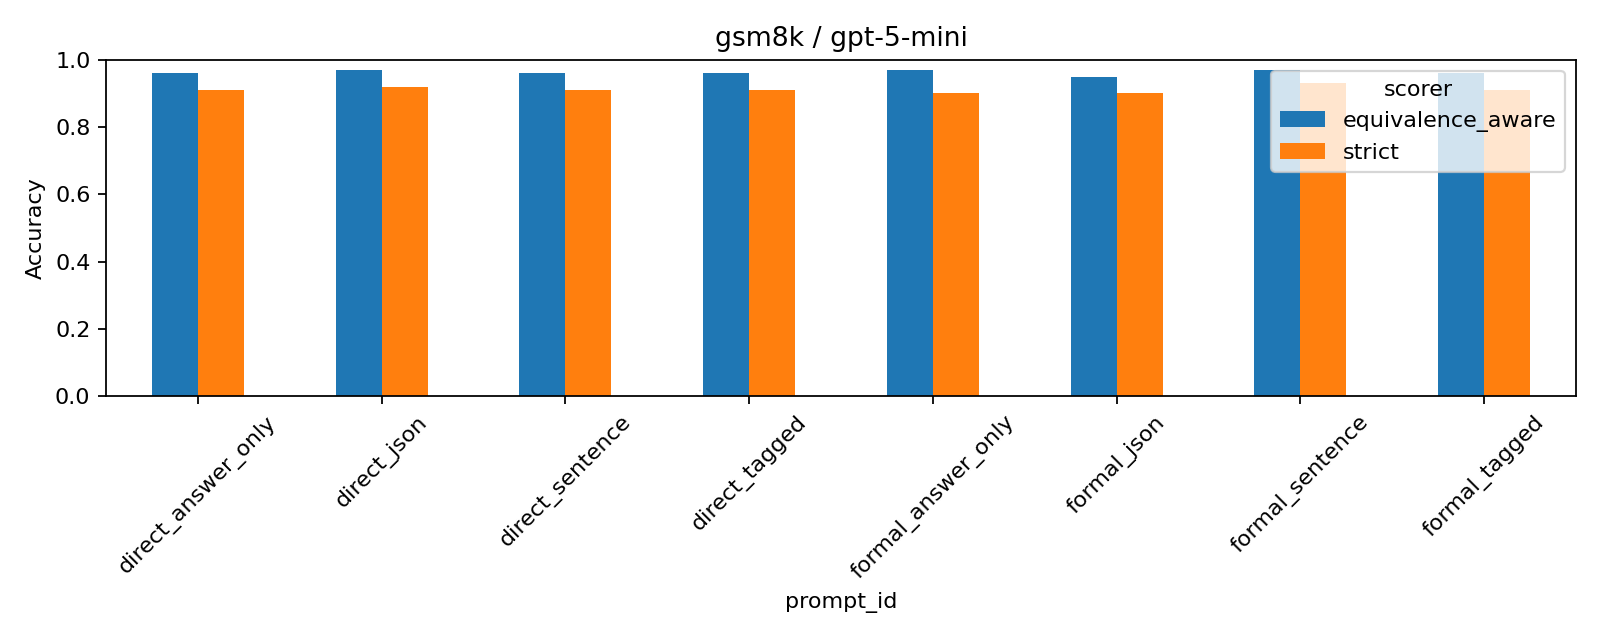
\includegraphics[width=\linewidth]{figures/accuracy_gsm8k_gpt-5-mini.png}
    \caption{GSM8K, \texttt{gpt-5-mini}}
\end{subfigure}
\hfill
\begin{subfigure}{0.48\linewidth}
    \centering
    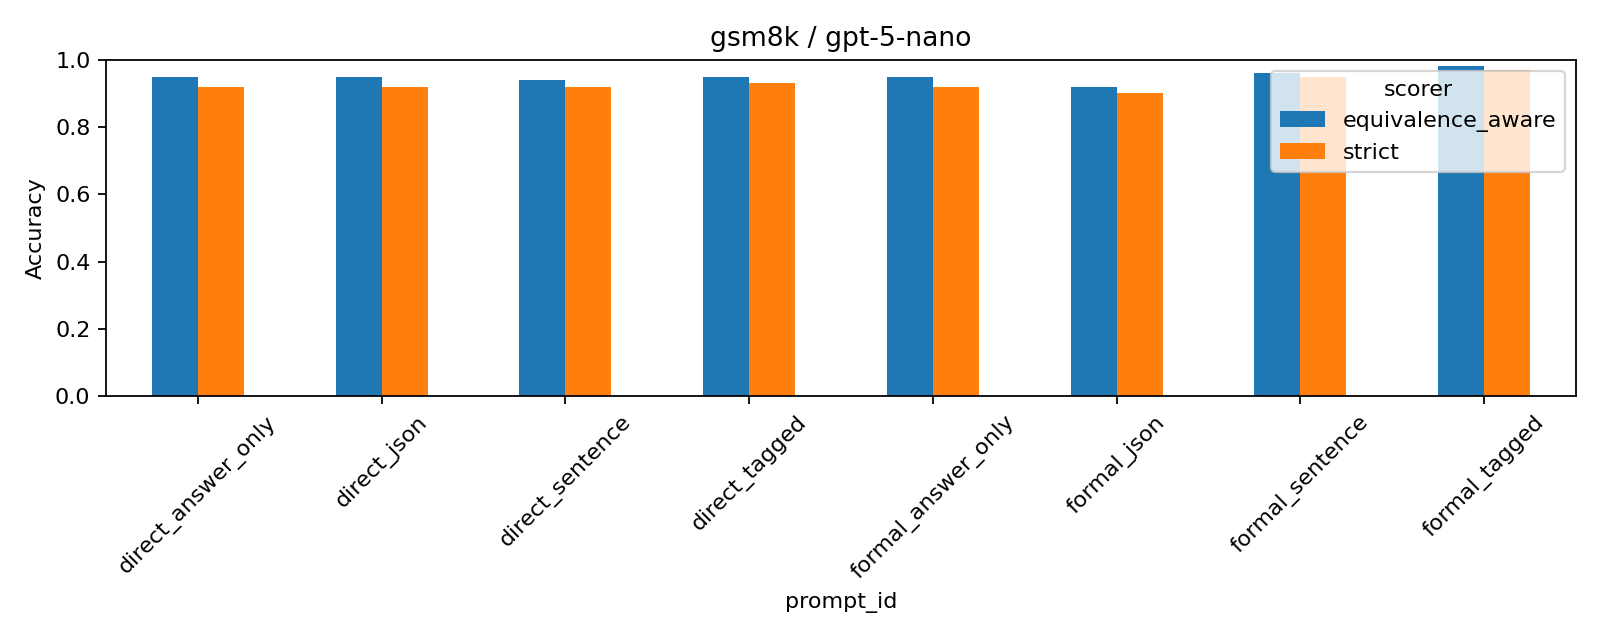
\includegraphics[width=\linewidth]{figures/accuracy_gsm8k_gpt-5-nano.png}
    \caption{GSM8K, \texttt{gpt-5-nano}}
\end{subfigure}
\caption{Prompt-level accuracy on GSM8K.}
\label{fig:gsm8k}
\end{figure}

\begin{figure}[t]
\centering
\begin{subfigure}{0.48\linewidth}
    \centering
    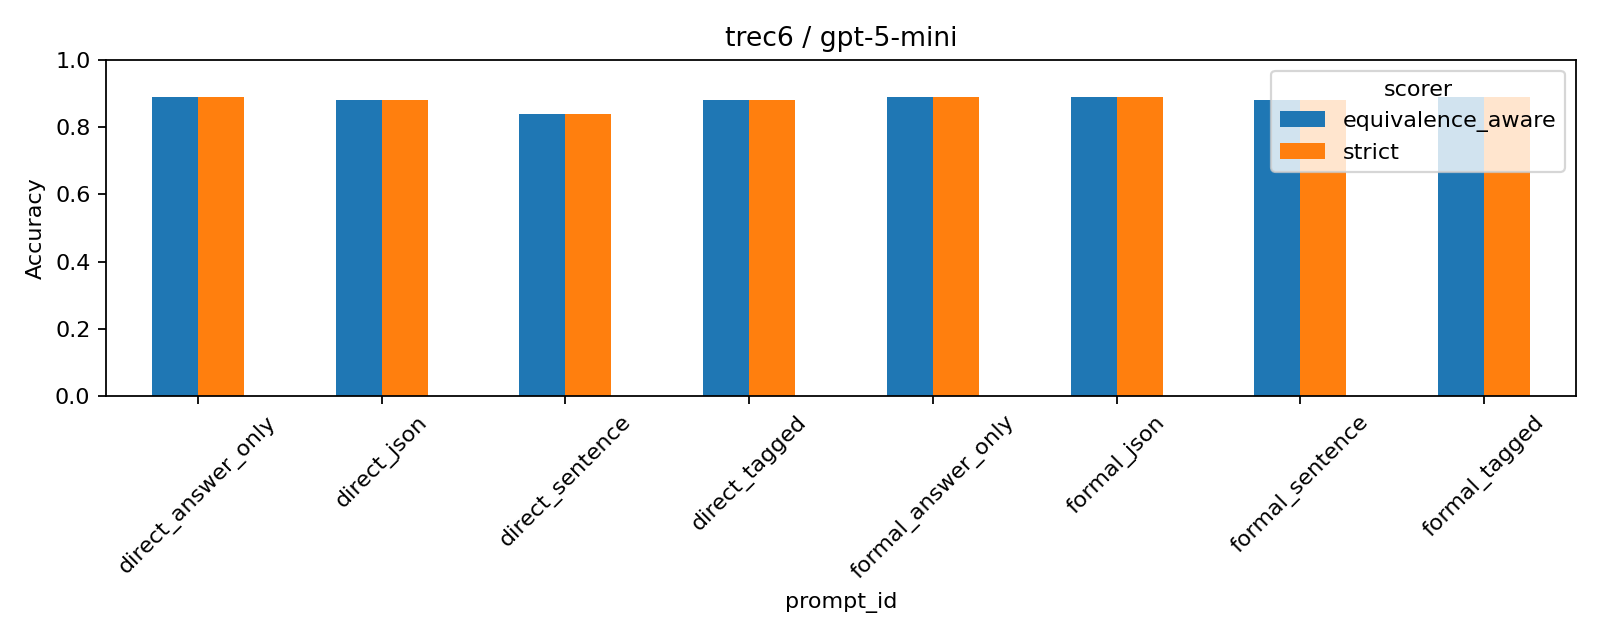
\includegraphics[width=\linewidth]{figures/accuracy_trec6_gpt-5-mini.png}
    \caption{TREC-6, \texttt{gpt-5-mini}}
\end{subfigure}
\hfill
\begin{subfigure}{0.48\linewidth}
    \centering
    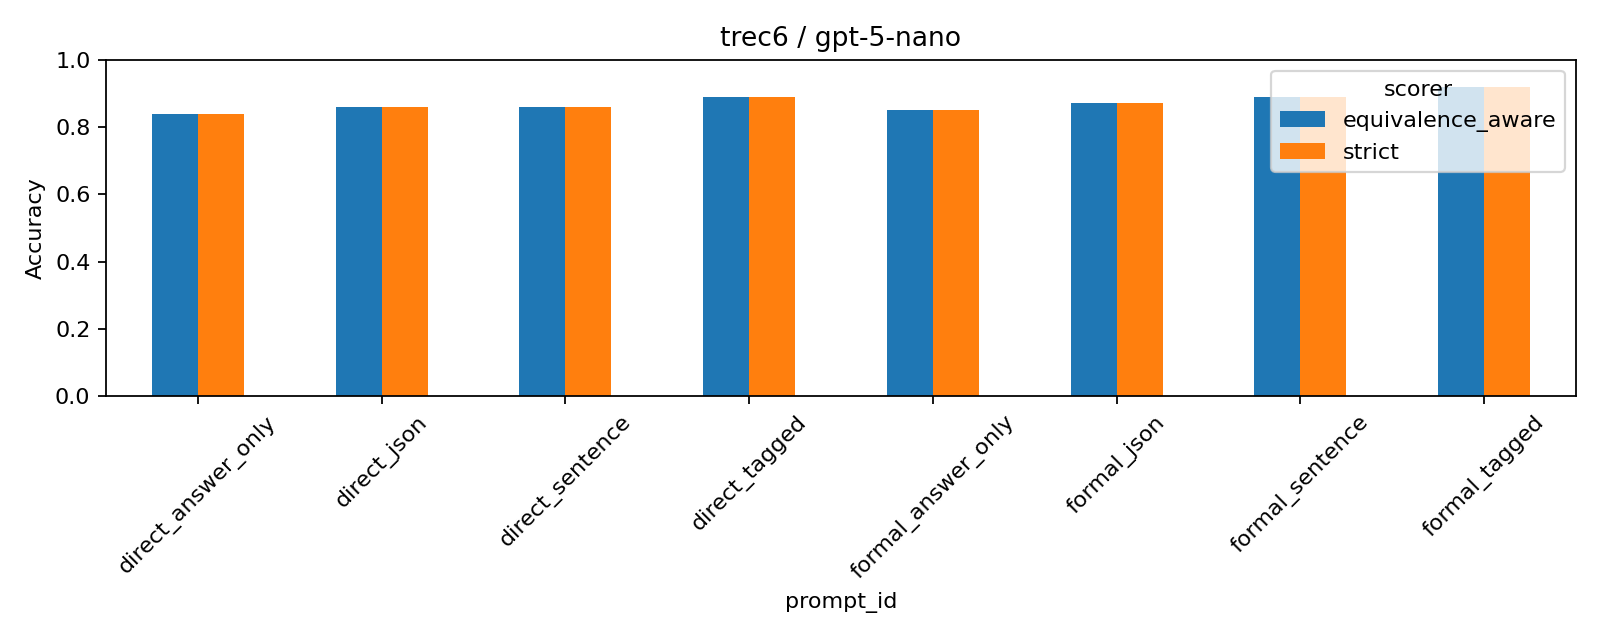
\includegraphics[width=\linewidth]{figures/accuracy_trec6_gpt-5-nano.png}
    \caption{TREC-6, \texttt{gpt-5-nano}}
\end{subfigure}
\caption{Prompt-level accuracy on TREC-6.}
\label{fig:trec}
\end{figure}

\subsection{Scorer Recoveries}

Across all 3,200 outputs, 326 fail strict scoring. The equivalence-aware scorer recovers 58 of these. All 58 recoveries occur on GSM8K. Of these, 41 are from \texttt{gpt-5-mini} and 17 are from \texttt{gpt-5-nano}. Typical recoveries involve numeric formatting:

\begin{itemize}[leftmargin=*]
    \item gold \texttt{5}, output \texttt{5.00};
    \item gold \texttt{5,600}, output \texttt{5600};
    \item gold \texttt{2}, output \texttt{\$2.00};
    \item gold \texttt{826}, output \texttt{826.00}.
\end{itemize}

These are not reasoning differences. They are evaluation-format artifacts. Strict scoring marks them wrong because the string differs from the gold answer or requested format, while the equivalence-aware scorer correctly treats them as numerically equivalent.

\section{LLM-Judge Audit}

The \texttt{gpt-5.4} judge audit covers every output with \texttt{strict\_correct = false}. This includes both outputs recovered by the rule-based equivalence-aware scorer and outputs rejected by both deterministic scorers.

\begin{table}[h]
\centering
\begin{tabular}{llrrrr}
\toprule
Task & Model & Judged & Rule Equiv. & Judge Equiv. & Agreement \\
\midrule
GSM8K & \texttt{gpt-5-mini} & 71 & 41 & 41 & 100\% \\
GSM8K & \texttt{gpt-5-nano} & 57 & 17 & 17 & 100\% \\
TREC-6 & \texttt{gpt-5-mini} & 96 & 0 & 0 & 100\% \\
TREC-6 & \texttt{gpt-5-nano} & 102 & 0 & 0 & 100\% \\
\bottomrule
\end{tabular}
\caption{LLM-judge audit over all strict-false outputs.}
\label{tab:judge}
\end{table}

The judge produces no parse failures and agrees exactly with the deterministic equivalence-aware scorer. It does not recover any additional cases rejected by the rule-based scorer, and it does not reject any cases recovered by the rule-based scorer. This supports the adequacy of the deterministic scorer for these two structured short-answer tasks.

\section{Error Analysis}

\paragraph{GSM8K.}
GSM8K errors mostly fall into two categories. The first is genuine wrong-answer behavior, where the model outputs an incorrect final number. The second is harmless numeric formatting, where strict scoring fails but equivalence-aware scoring succeeds. The latter category is exactly the scoring artifact targeted by this project.

The prompt sensitivity on GSM8K is modest but nonzero. For \texttt{gpt-5-nano}, strict prompt accuracy ranges from 90\% to 97\%. The best-performing prompt is \texttt{formal\_tagged}, while \texttt{formal\_json} is lowest. This suggests that output constraints can interact with model behavior, although the effect is not large in this setting.

\paragraph{TREC-6.}
TREC-6 errors are primarily label confusions. For example, questions whose answer type is an entity can be confused with descriptions, and location-seeking questions can be confused with entity labels when the target answer is a named object such as a mountain range. Because the output space is a small label set, the equivalence-aware scorer has little to recover beyond minor label aliases. This explains why strict and equivalence-aware scoring produce identical TREC-6 results.

\paragraph{Token-cap cleanup.}
During the first main run, 14 \texttt{gpt-5-nano}/GSM8K responses hit the maximum output-token cap and returned empty outputs. These records were retried with a larger output-token cap and merged into the clean final run. The final reported results use only the cleaned run, which has 3,200 completed outputs and no empty responses.

\section{Limitations}

This project is intentionally scoped. It uses only two tasks, two OpenAI models, and 100 examples per task. The prompt family is controlled and interpretable, but it is not exhaustive. Other prompt paraphrases, few-shot settings, or reasoning-style prompts could produce different sensitivity patterns.

The equivalence-aware scorer is deterministic and task-specific. This is a strength for reproducibility, but it limits generality. It is appropriate for TREC-6 labels and GSM8K numeric answers, but would not directly transfer to open-ended generation. The LLM-judge audit helps validate the scorer in this setting, but it is not a substitute for human evaluation.

The experiment also uses provider-default reasoning and decoding behavior. This reflects normal API use, but it means hidden reasoning-token behavior is not fully controlled. Finally, because the evaluated models are from a single provider, the results should not be interpreted as a broad cross-provider robustness claim.

\section{Conclusion}

This project re-tests prompt and output-format sensitivity on modern LLMs in a small controlled setting and adds a scoring-method ablation. The results show moderate prompt sensitivity across both tasks and models. The observed sensitivity is not purely a scoring artifact: prompt-level accuracy still varies after equivalence-aware scoring. However, scoring artifacts are present on GSM8K, where strict matching undercounts semantically correct numeric outputs with harmless formatting differences. TREC-6 shows no strict-versus-equivalence gap because the outputs are usually canonical labels or genuinely wrong labels.

The LLM-judge audit agrees exactly with the deterministic equivalence-aware scorer on all strict-false cases, suggesting that the rule-based scorer is adequate for these structured tasks. Overall, the results support a pragmatic conclusion: multi-prompt evaluation remains useful, and scoring definitions materially affect measured performance when tasks admit benign output variation.

\appendix

\section{Prompt Templates}

The exact prompt consists of a wording instruction, the task input, and an output-format instruction.

\subsection{Instruction Wordings}

TREC-6 direct:

\begin{quote}
Classify the question into exactly one of these labels: ABBR, ENTY, DESC, HUM, LOC, NUM.
\end{quote}

TREC-6 formal:

\begin{quote}
Assign the coarse question type for the item below. The valid labels are ABBR, ENTY, DESC, HUM, LOC, and NUM.
\end{quote}

GSM8K direct:

\begin{quote}
Solve the math problem.
\end{quote}

GSM8K formal:

\begin{quote}
Determine the final numerical answer for the grade-school math problem below.
\end{quote}

\subsection{Output-Format Instructions}

TREC-6:

\begin{itemize}[leftmargin=*]
    \item Answer only: Return only the label, with no extra text.
    \item Sentence: Return exactly one sentence in this form: The answer is \verb|<label>|.
    \item Tagged: Return the answer inside XML tags in this form: \verb|<answer>LABEL</answer>|.
    \item JSON: Return valid JSON in this form: \verb|{"answer": "<label>"}|.
\end{itemize}

GSM8K:

\begin{itemize}[leftmargin=*]
    \item Answer only: Return only the final number, with no extra text.
    \item Sentence: Return exactly one sentence in this form: The answer is \verb|<number>|.
    \item Tagged: Return the answer inside XML tags in this form: \verb|<answer>NUMBER</answer>|.
    \item JSON: Return valid JSON in this form: \verb|{"answer": "<number>"}|.
\end{itemize}

\section{Scoring Details}

The strict scorer is deliberately brittle. It requires exact format compliance and exact answer equality. The equivalence-aware scorer parses JSON, XML-style tags, answer sentences, and raw outputs. For TREC-6, it canonicalizes labels and a small alias set. For GSM8K, it extracts numeric answers and compares exact decimal values after removing commas, currency symbols, trailing periods, and whitespace.

\section{Reproducibility Artifacts}

The final committable results are stored under:

\begin{itemize}[leftmargin=*]
    \item \texttt{reports/results/main\_clean/}
    \item \texttt{reports/results/full\_outputs/}
    \item \texttt{reports/results/judge\_audit\_gpt54/}
\end{itemize}

The full clean output set contains 3,200 records. The LLM-judge audit contains 326 judged records.

\bibliographystyle{plainnat}
\bibliography{references}

\end{document}
